\documentclass[a4paper,12pt,oneside]{book}

%-------------------------------Start of the Preable------------------------------------------------
\usepackage[english]{babel}
\usepackage{blindtext}
%packagr for hyperlinks
\usepackage{hyperref}
\usepackage{subcaption}
\usepackage{caption}
\usepackage{float}
\hypersetup{
    colorlinks=true,
    linkcolor=blue,
    filecolor=magenta,      
    urlcolor=cyan,
}

\urlstyle{same}
%use of package fancy header
\usepackage{fancyhdr}
\setlength\headheight{26pt}
\fancyhf{}
%\rhead{
\includegraphics[width=1cm]{logo}}
\lhead{\rightmark}
\rhead{
\includegraphics[width=1cm]{logo}}
\fancyfoot[RE, RO]{\thepage}
\fancyfoot[CE, CO]{\href{http://www.e-yantra.org}{www.e-yantra.org}}

\pagestyle{fancy}

%use of package for section title formatting
\usepackage{titlesec}
\titleformat{\chapter}
  {\Large\bfseries} % format
  {}                % label
  {0pt}             % sep
  {\huge}           % before-code
 
%use of package tcolorbox for colorful textbox
\usepackage[most]{tcolorbox}
\tcbset{colback=cyan!5!white,colframe=cyan!75!black,halign title = flush center}

\newtcolorbox{mybox}[1]{colback=cyan!5!white,
colframe=cyan!75!black,fonttitle=\bfseries,
title=\textbf{\Large{#1}}}

%use of package marginnote for notes in margin
\usepackage{marginnote}

%use of packgage watermark for pages
%\usepackage{draftwatermark}
%\SetWatermarkText{
\includegraphics{logo}}
\usepackage[scale=2,opacity=0.1,angle=0]{background}
\backgroundsetup{
contents={
\includegraphics{logo}}
}

%use of newcommand for keywords color
\usepackage{xcolor}
\newcommand{\keyword}[1]{\textcolor{red}{\textbf{#1}}}

%package for inserting pictures
\usepackage{graphicx}

%package for highlighting
\usepackage{color,soul}

%new command for table
\newcommand{\head}[1]{\textnormal{\textbf{#1}}}


%----------------------End of the Preamble---------------------------------------


\begin{document}

%---------------------Title Page------------------------------------------------
\begin{titlepage}
\raggedright
{\Large eYSIP2018\\[1cm]}
{\Huge\scshape Low cost sensor node for wsn  \\[.1in]}
\vfill
\begin{center}
 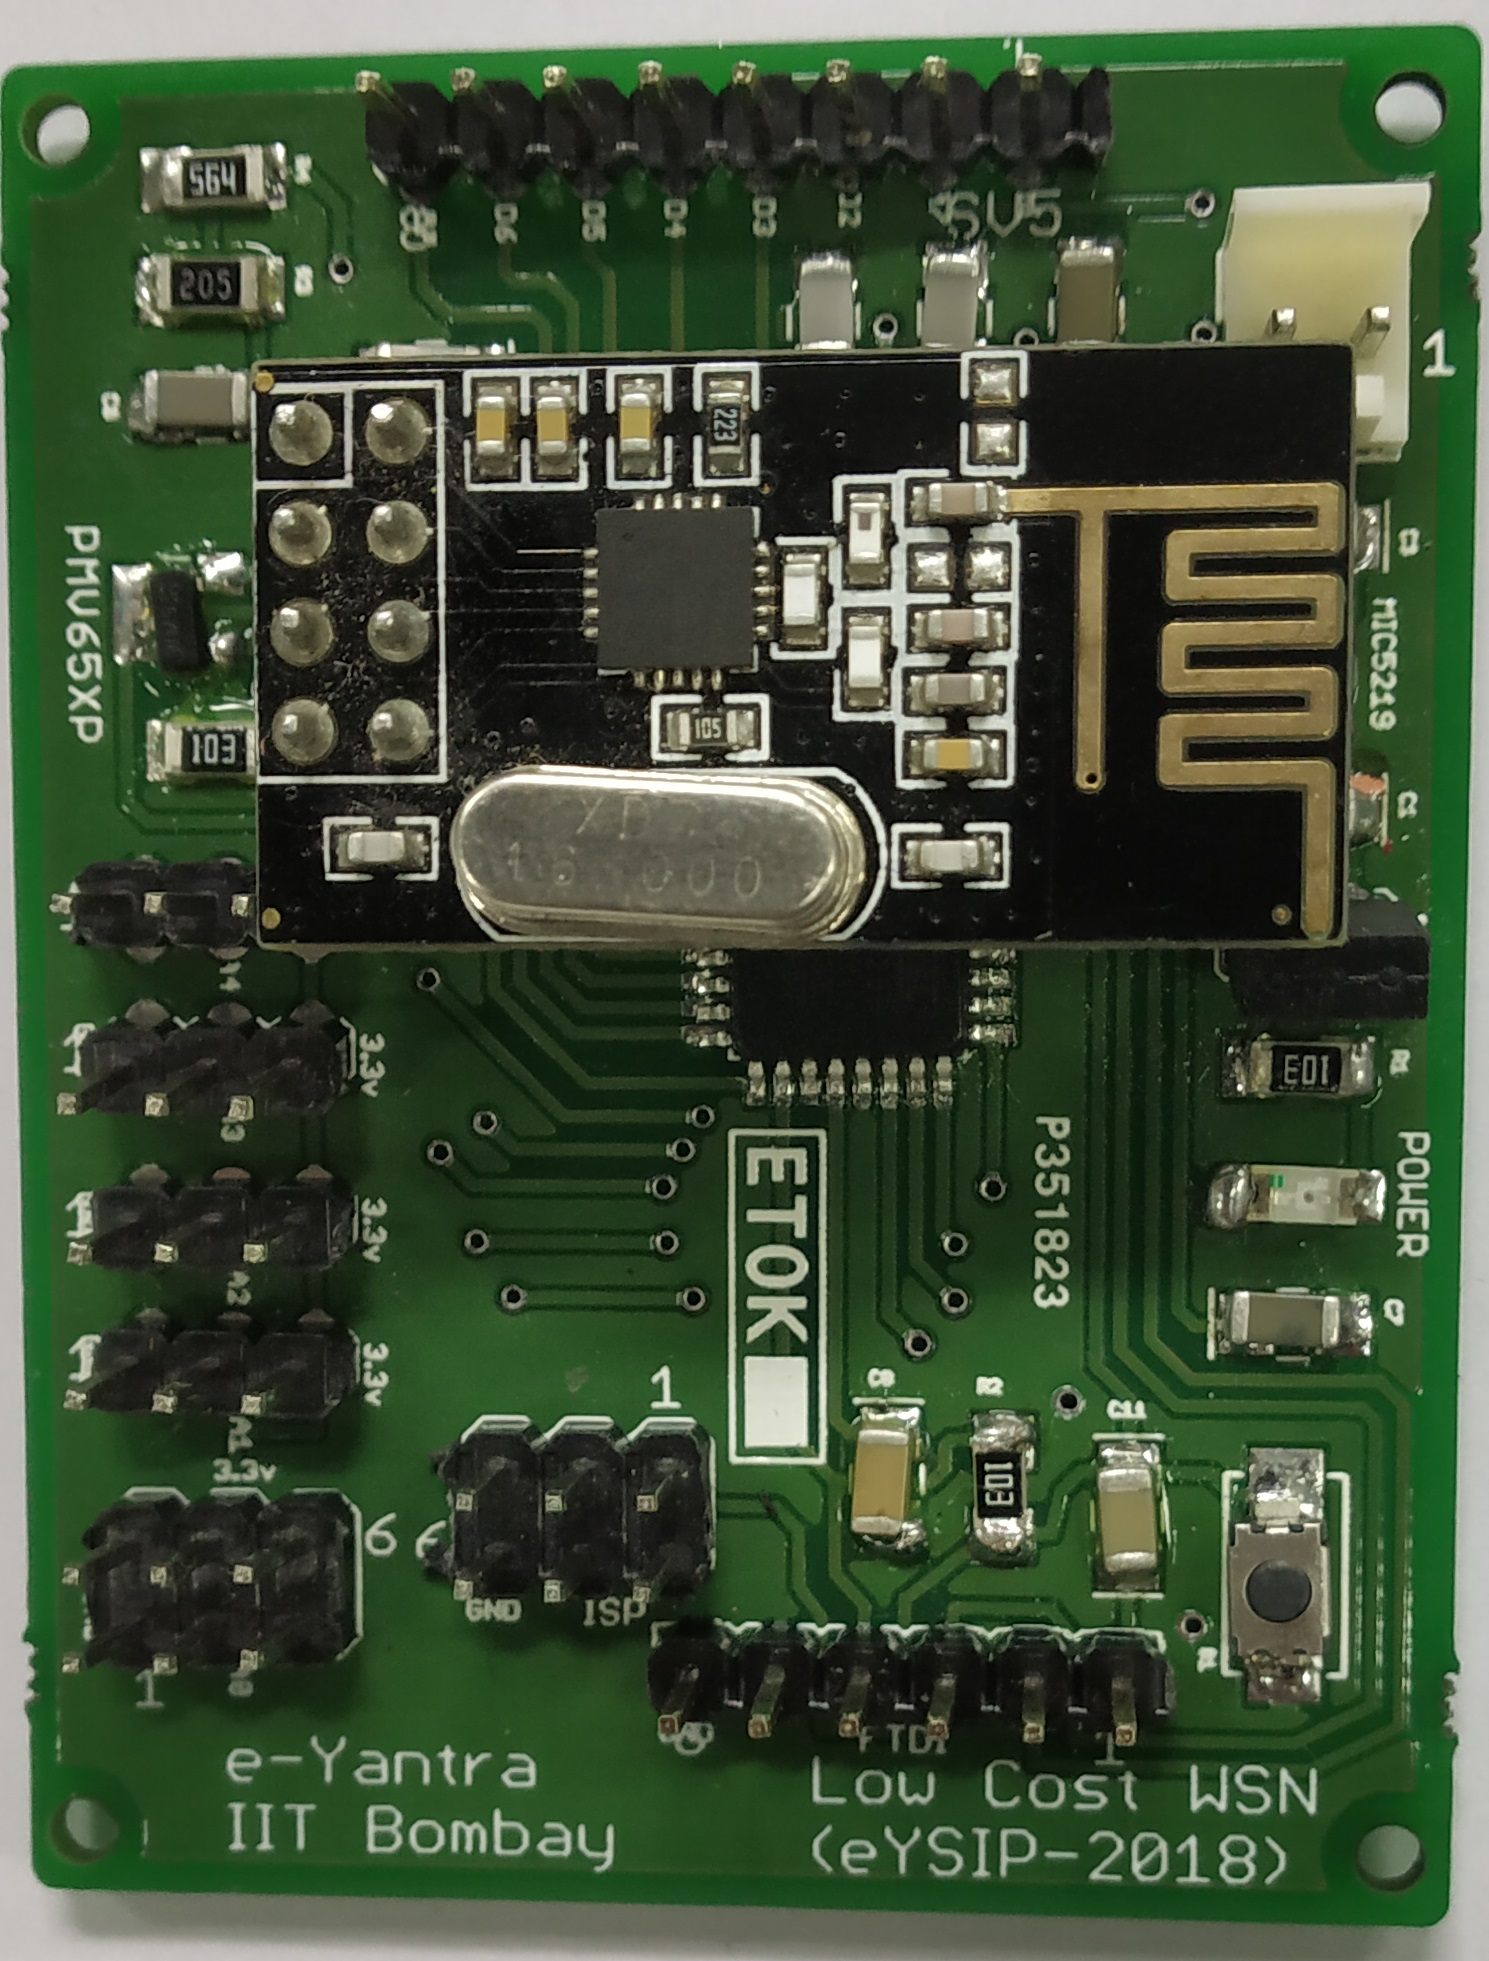
\includegraphics[width=0.6\textwidth]{node_Printed_board.PNG}
 \end{center}
\begin{flushright}
{\large Sachin Mahadev Jadhav \\}
{\large Nithin Thilakappan \\}
{\large Nishit Patel \\}
{\large  Parin Chheda \\}
{\large  Kalind Karia \\}
{\large Duration of Internship: $ 21/05/2018-06/07/2018 $ \\}
\end{flushright}

{\itshape 2018, e-Yantra Publication}
\end{titlepage}
%-------------------------------------------------------------------------------

\chapter[Project Tag]{Low cost sensor node for WSN}
\section*{Abstract}
The prime motive of this project is to make sensor node based on Atmega328 platform that has the
\\ Following features:
\begin{enumerate}
\item custom built power supply for optimized for low power sensor node applications
\item Ability to program via Arduino IDE/ Atmel Studio 
\item Use NRF2401 for RF communication
\item Completely open source design and sample codes to make it useful for WSNs
\item Can be used as general purpose microcontroller board for learning interfacing and C programming
\end{enumerate}

\subsection*{Completion status}
 

\section{Hardware parts}
\begin{itemize}
  \item List of hardware 
  \begin{enumerate}
  \item Atmega328p
  \item nRF24L01
  \item PMV65XP (MosFET)
  \item AP2112 (LDO)
  \item ESP32 (Gateway)
  \end{enumerate}
  \clearpage
  \item Detail of each hardware: 
       \begin{enumerate}
        \item \textbf{Atmega328p} is used as on board main microcontroller for each and every node due to its high performance and low power consumption. nRF24L01 is connected to its SPI bus for radio communication. Different types of sensors can be interfaced to its ADC port. Also its GPIO pins are taken out on the board so that board can be used as a microcontroller development board for testing purpose.
\href{http://ww1.microchip.com/downloads/en/DeviceDoc/Atmel-42735-8-bit-AVR-Microcontroller-ATmega328-328P_Datasheet.pdf}{Atmega328p Datasheet},
        \href{https://www.amazon.in/Microcontroller-Atmega328P-Au-Tqfp-32-Atmel-Chip/dp/B004ZV92TA?tag=googinhydr18418-21&tag=googinkenshoo-21&ascsubtag=038287ef-bfda-4a20-8b15-785c3e8b240c}{Vendor link}
        \item \textbf{nRF24L01} is used to send data via radio communication between each nodes. The \textbf{nRF24L01} is a single chip \textbf{2.4GHz transceiver} with an embedded baseband protocol engine
(Enhanced ShockBurst™), designed for ultra low power wireless applications. The textbf{nRF24L01} is designed
for operation in the world wide ISM frequency band at \textbf{2.400 - 2.4835GHz.} An MCU (microcontroller) and
very few external passive components are needed to design a radio system with the \textbf{nRF24L01.}
The \textbf{nRF24L01} is configured and operated through a Serial Peripheral Interface (SPI.) Through this interface
the register map is available. The register map contains all configuration registers in the \textbf{nRF24L01}
and is accessible in all operation modes of the chip.
The embedded baseband protocol engine (Enhanced ShockBurst™) is based on packet communication
and supports various modes from manual operation to advanced autonomous protocol operation. Internal
FIFOs ensure a smooth data flow between the radio front end and the system’s MCU. Enhanced ShockBurst™
reduces system cost by handling all the high-speed link layer operations.
         \href{https://www.nordicsemi.com/eng/content/download/2730/34105/file/nRF24L01_Product_Specification_v2_0.pdf}{nRF24L01 Datasheet},
  \href{https://robu.in/product/m177-nrf24l01-2-4ghz-antenna-wireless-transceiver-module/?gclid=Cj0KCQjwvezZBRDkARIsADKQyPknzJJk923OEc9ihJ7ZoGdwvh2pjVOp52CF125ixwnoAMcel50iYmwaAuKoEALw_wcB}{Vendor link}     

\item \textbf{PMV65XP} is P-channel enhancement mode Field-Effect Transistor (FET) in a small SOT23
(TO-236AB) Surface-Mounted Device (SMD) plastic package using Trench MOSFET
technology.
\begin{itemize}
\item Low threshold voltage 
\item Low on-state resistance
\item Trench MOSFET technology
\end{itemize}
\href{https://assets.nexperia.com/documents/data-sheet/PMV65XP.pdf}{PMV65Xp Datasheet},
  \href{https://www.digikey.in/product-detail/en/nexperia-usa-inc/PMV65XP215/1727-3124-1-ND/949693}{Vendor link}     


\item  The  \textbf{AP2112}  is  CMOS  process  low  dropout  linear  regulator  with 
enable  function,  the  regulator  delivers  a  guaranteed  600mA  (min.) 
continuous load current. 
        \href{https://www.diodes.com/assets/Datasheets/AP2112.pdf}{AP2112 Datasheet},
        \href{https://www.mouser.in/Search/Refine.aspx?Keyword=AP2112}
        {Vendor link} 
        \item \textbf{ESP32} is a single 2.4 GHz Wi-Fi-and-Bluetooth combo chip designed with the TSMC ultra-low-power 40 nm
technology. It is designed to achieve the best power and RF performance, showing robustness, versatility and
reliability in a wide variety of applications and power scenarios. \href{https://www.espressif.com/sites/default/files/documentation/esp32_datasheet_en.pdf}{ESP32 Datasheet}, \href{https://robokits.co.in/iot-internet-of-things/esp32-development-board-wifi-bluetooth?gclid=CjwKCAjwj4zaBRABEiwA0xwsPzdTv88ACYXS8xP16QkXnavkAI1VsyFrMKXILtADRV6BI9Ox5uXtXxoCw5MQAvD_BwE&zenid=2e2v1a2o33svqkk9gdknbbgbt5}
        {Vendor link} 
 

        
        \end{enumerate}
  \end{itemize}
  \begin{itemize}
   \item PCB schematic design of circuit
         
   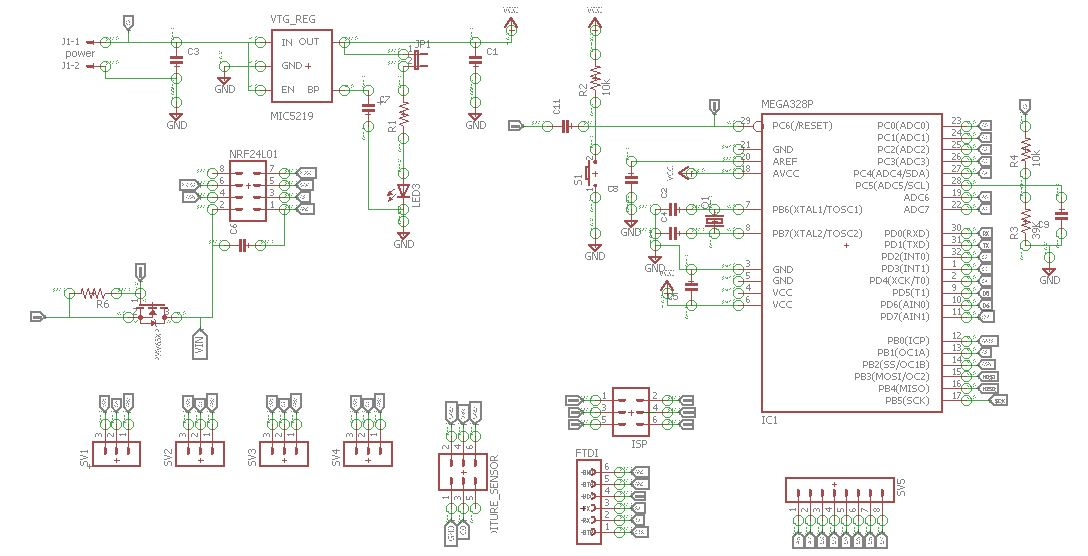
\includegraphics[width=1\textwidth]{eagle_sch_snap.JPG}\\
         \begin{center}
         \small{Figure 1\textbf{. Schematic Diagram}}
\end{center}
  
\end{itemize}

\section{Software Used}
\begin{itemize}
  \item List of software used
  \begin{enumerate}
  \item Arduino IDE
  \item Atmel Studio IDE
  \end{enumerate}
  \item Detail of software:
  \begin{enumerate}
  \item \textbf{Arduino IDE} is used for programming the main microcontroller atmega328p as per user requirement. version 1.8.5
  \href{https://www.arduino.cc/en/Main/Software?}{Arduino IDE download}
  \item \textbf{Atmel Studio 7.0}
  \href{http://studio.download.atmel.com/7.0.1931/as-installer-7.0.1931-full.exe}{download}
  \end{enumerate}
  \clearpage
  \item Installation steps
  \begin{enumerate}
  \item Instruction for installation of \textbf{Arduino IDE 1.8.5}
  \href{https://learn.sparkfun.com/tutorials/installing-arduino-ide}{click here}
  \item Instruction for installation of \textbf{Atmel Studio IDE 7.0} \href{http://ww1.microchip.com/downloads/en/DeviceDoc/Getting-Started-with-Atmel-Studio7.pdf}{click here}
  \end{enumerate} 
\end{itemize}
\section{Set up and Programming}
\subsection*{Setting up fusebits on atmega328p}
\begin{itemize}
\item NEX AVR USB ISP STK500V2 is used for setting up fusebits and flashing program files into the microcontroller because of its high speed.
In-System USB programmer for AVR family of microcontrollers. It can be used with
AVR Studio on Win XP platforms. 
\item For Windows 7 and Windows 10 it can be used in HID
mode with Avrdude command prompt as programming interface. Its adjustable clock
speed allows programming of microcontrollers with lower clock speeds. 

\item Using HID mode of stk500v2 does not require any driver installation before we start to use it. 
Because it uses generic windows drivers.
\item Download necessary files of AVRdude to run the programmer in HID mode \href{http://www.nex-robotics.com/images/downloads/NEX\%20AVR\%20STK500V2.zip}{click to download}
\item After downloading necessary files from above link \href{http://www.nex-robotics.com/images/downloads/avr\%20usb\%20programmer\%20manualv2_.pdf}{click here} for basic setup and installation refer page 19 and 20.
\item TO know more about AVRDUDE commands 
\href{https://drive.google.com/file/d/1mJsKZGY1hJlm7xWhdA7beEfMs0qJASh_/view}{AVRDude Commands meaning}
\item \textbf{Steps for setting up fusebits using stk500v2 commands}

\begin{enumerate}
\item \textbf{Show default settings all Fuse bits, lock bits ,mode of programming of microcontroller}\\
 avrdude -c stk500v2 -p m328p -P NEX-USB-ISP -v
 \item \textbf{Modifying the default fusebits}\\
 avrdude -c stk500v2 -p m328p -P NEX-USB-ISP -U efuse:w:0x05:m -U hfuse:w:0xda:m -U lfuse:w:0xff:m
 \item \textbf{Uploading a program file(.hex file) into microcontroller}\\
 avrdude -c stk500v2 -p m328p -P NEX-USB-ISP -U flash:w:codename.hex
  \item \textbf{setting of lock bits}\\
 avrdude -c stk500v2 -p m328p -P NEX-USB-ISP -U lock:w:ox0f:m

\end{enumerate}

\end{itemize}

\subsection*{Burning bootloader into atmega328p}

\begin{itemize}
\item \href{https://learn.sparkfun.com/tutorials/installing-an-arduino-bootloader}{Click here} to refer steps for burning a bootloader 
\item Bootloader which we used was from a arduino directory i.e., local disk C: then Program Files (x86) then Arduino then hardware then arduino then avr then bootloaders then atmega then ATmegaBOOT168atmega328pro8MHz.hex 
\end{itemize}
\section{Assembly of hardware}

\subsection*{Block Diagram}
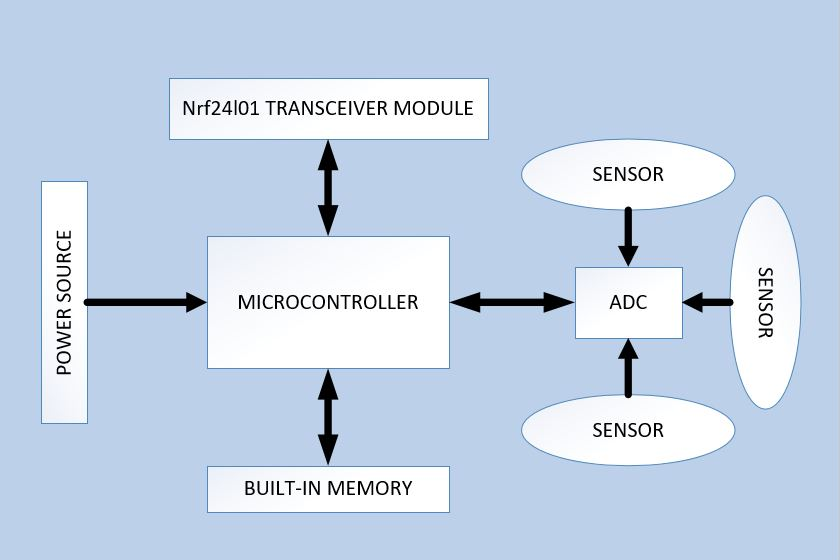
\includegraphics[width=1\textwidth]{block_diagram_node.JPG}
\begin{center}
         \small{Figure 2\textbf{. Block diagram of system}}
\end{center}
\clearpage

\begin{figure}[H]
\centering
\begin{subfigure}{0.5\textwidth}
\centering
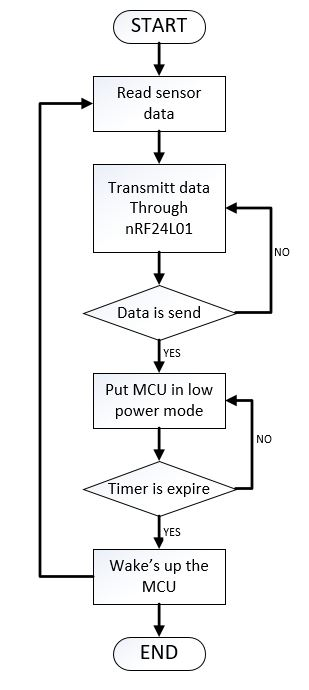
\includegraphics[width=0.5\linewidth]{trance_flow_snap.JPG}
\caption{Transmitter flow chart}
\end{subfigure}
\begin{subfigure}{0.5\textwidth}
\centering
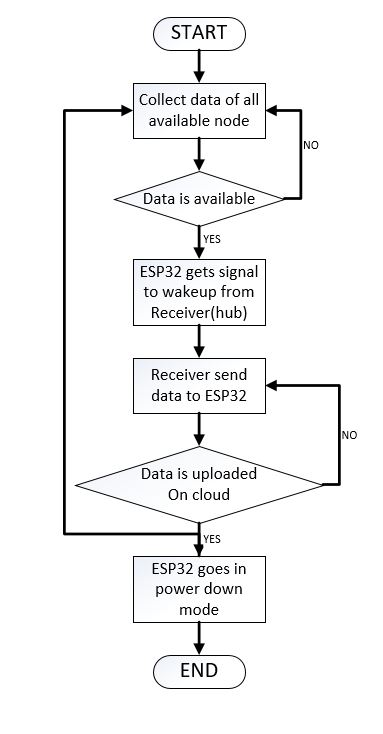
\includegraphics[width=0.50\linewidth]{receiver_flow_snap.JPG}
\caption{Receiver flow chart}
\end{subfigure}
\end{figure}
\label{Figure 3. Flow chart}
\begin{itemize}
\item This project was mainly concentrated on urban farming where the sensor node will keep monitoring the farming parameters which should be taken an immense attention towards it
\item  So  multiple sensors will be placed at different locations from where it will send parameters like soil moisture data, temperature data, humidity data etc
\item  By including multiple sensor nodes into the field it will create a network through which it will communicate with each other and data will the received at a hub point and from the hub point there is an ESP32 module acting as a gateway of this network for uploading the received data to the internet i.e., thingspeak cloud. It is possible to implement different type of network as per the complexity of the requirement and how much distance is to be covered
\item Types of network are
\begin{enumerate}
\item  Star network
\item Mesh network
\item Hybrid network
\end{enumerate}
\item  Here we have implemented a star network completely on the c language which means we developed the required libraries which is used in the star network
\item Parallel to that we have also implemented the whole system in mesh network too but we are using arduino libraries for the same c language libraries is remaining to be developed.
\end{itemize}

\subsection*{\textbf{Implementation of mesh network using three  sensor nodes and an esp32 module.}}

  \begin{center}
     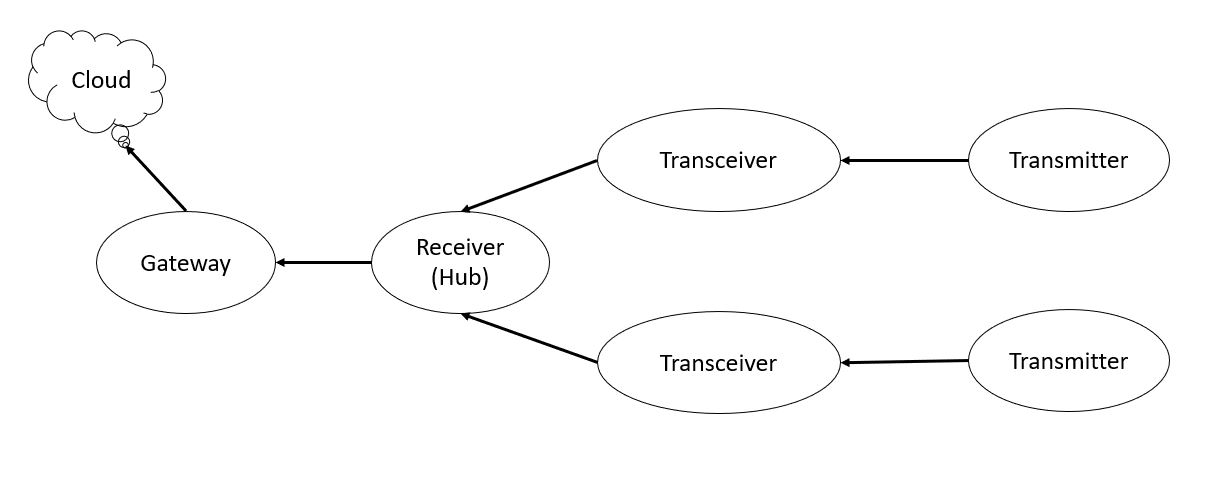
\includegraphics[width=0.83\textwidth]{mesh_diagram.JPG}\\
         \small{Figure 3\textbf{. Flow diagram of mesh network}}
   \end{center}
         
\begin{itemize}
\item Those three nodes were given a particular node number like node 1, node 2, node 3 here node one is  a transmitter node 2 is an intermediate transceiver node and node number 3 is said to be an hub of the network which is serially connected with the ESP32. Out of three sensor nodes node number one was not in the range of node 3 so we kept an intermediate node 2 in between node 1 and node 3 so that data from node 1 can be transmitted to node 3 via node 2.
\item Initially node 1 and node 2 with be in sleep mode it will wake up at every 20 seconds to transmit it's data to the hub node 3. At the time of data transmission node 1 wakes up and transmit it's data to node 2 and node 2 wake up and receive the data of node 1 and it will send it's own data along with the received data from node 1 to the hub node 3 from node 3 it will be serially transmitted to the ESP32 module which will upload the data to the thingspeak server.
\end{itemize}


\textbf{How does ESP32 (Gateway) works?}

\begin{itemize}
\item Here ESP32 is used along with an NRF based receiver to act as a gateway. 
\item ESP32 is connected with receiver (hub) via serial UART2 (RX, TX) for serial Communication. 
\item Normally ESP32 will be in a sleep mode as soon as when the hub receives all the data's from all  the nodes it will send an interrupt signal to the ESP32 to wakeup from the sleep mode and setup a wlan connection through WiFi and connect to the thingspeak server. 
\item After setting up a successful connection with the server, then it will send an acknowledgement to the receiver hub regarding the setup of connection. 
\item As soon as the acknowledgement is received at the hub, hub will send all the data to the ESP32 via serial Communication, while the data is received at ESP32 it will ask for a post request on the thingspeak server through which the data will be uploaded to the thingspeak server.
    \item Measure current of PCB board
    \begin{itemize}
    	\item Transmit mode current = \textbf{6.7 mA}
        \item Receiver mode current = \textbf{22-25mA}
        \item Sleep mode current = \textbf{100 uA}
       
    \end{itemize}
    \item Measure current of nRF24L01
    \begin{itemize}
    	\item Normal mode current = \textbf{1.2 mA}  
        \item stand by mode current = \textbf{40 uA}
        \item Sleep mode current = \textbf{900 nA}
    \end{itemize}
    \clearpage
    \item Current measurement of Pcb board and nRF24L01 on DSO
     \begin{center}
     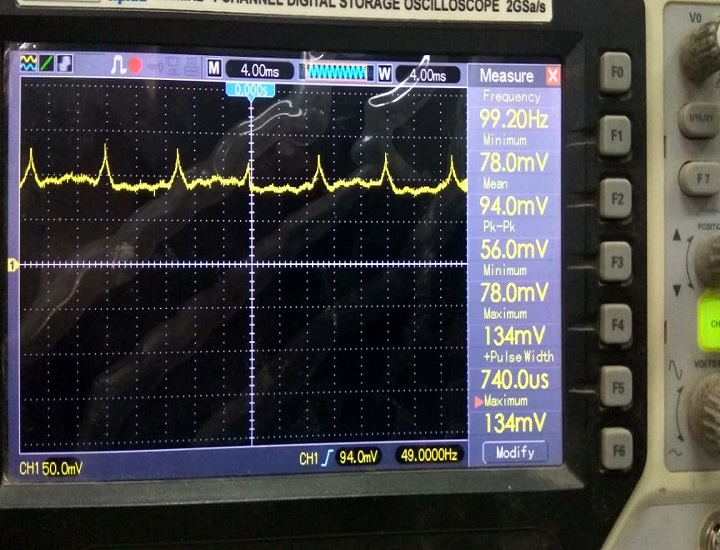
\includegraphics[width=0.83\textwidth]{main_transmitt.PNG}\\
         \small{Figure 4\textbf{. Current of PCB Board (transmit mode(6.7mA))}}
         
     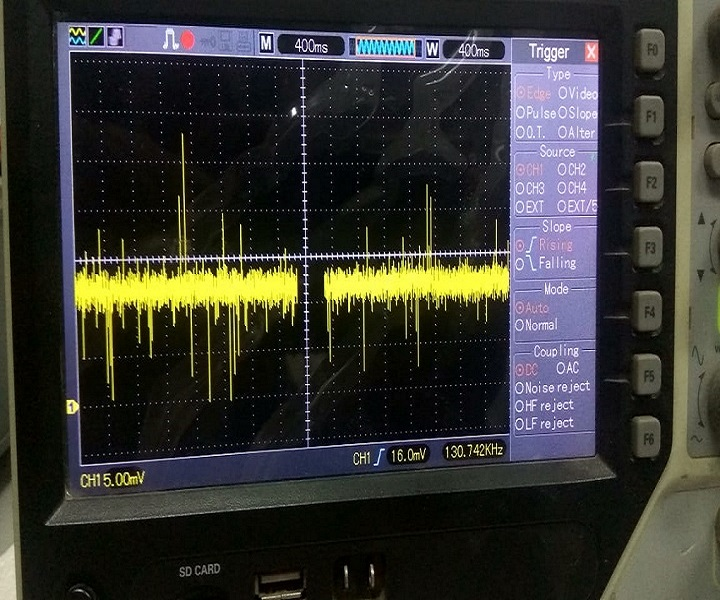
\includegraphics[width=0.83\textwidth]{main_receiver.PNG}\\
         \small{Figure 5\textbf{. Current of PCB Board (receiver mode(22-25mA))}}\\
        \end{center}
    \item Test the range of nRF24L01 in outdoor environment with different data rate
    \begin{itemize}
    	\item  MIN (-18 dBm) power = \textbf{0 to 6 m}
        \item  LOW (-12 dBm) power = \textbf{0 to 8 m}
        \item  HIGH (-6 dBm) power = \textbf{0 to 12 m}
        \item  MAX (0 dBm) power = \textbf{0 to 16 m}
	\end{itemize}
    \end{itemize}
\begin{table}[!h]
\centering
  \caption{Range testing of nRF24L01 (At different data rates)}
    \begin{tabular}{|c|c|c|c|c|}
    \hline
    \multicolumn{1}{| p{5.715em} |}{Transmission \newline{}Power level} & \multicolumn{1}{ | p{3.715em} | }{MIN power\newline{}(-18 dBm)} & \multicolumn{1}{| p{4em} |}{LOW power\newline{}(-12 dBm)} & \multicolumn{1}{| p{4.145em} |}{HIGH power \newline{}(-6 dBm)} & \multicolumn{1}{|p{3.855em}|}{MAX power \newline{}(0 dBm)} \\
    \multicolumn{1}{|l|}{Distance (meter)} & & & & \\\hline
    3.8   & 100\% & 100\% & 100\% & 100\% \\\hline
    4.9   & 100\% & 100\% & 100\% & 100\% \\\hline
    5.9   & 100\% & 100\% & 100\% & 100\% \\\hline
    6.9   & 47\%  & 100\% & 100\% & 100\% \\\hline
    8     & 0\%   & 100\% & 100\% & 100\% \\\hline
    8.2   & 0\%   & 100\% & 100\% & 100\% \\\hline
    10    & 0\%   & 74\%  & 100\% & 100\% \\\hline
    12.4  & 0\%   & 0\%   & 100\% & 100\% \\\hline
    15.6  & 0\%   & 0\%   & 86\%  & 100\% \\\hline
    \end{tabular}
  \label{tab:addlabel}
\end{table}
\begin{itemize}
\item 100\% means after transmitting 15 packets from transmitter side all 15 packets have successfully received at receiver end.
\item Range testing was carried out at the terrace of KReSiT building where there was greenery because of the farming carried out over there also there was few wifi routers functioning nearby the farming area which forced us to use a different radio communication channel number i.e., 76 which won't be effected by the wifi networks.
\item As we know that greenery absorbs 2.4 GHz frequency due to which some of our data packets failed to receive at receiver end in some conditions.
\item As shown in the above table 3.8- 5.9 meters distance communication is completely working very well in all the power levels of nRF24L01.
\item While increasing the distance at 6.9 meters the received packets were moderate which is 47 percent of 15 packets.
\item Again testing nRF24L01 to its extreme level the distance was kept 15.6 meters and the complete packets received at receiver end only in max power level rest all other modes failed.
 
\end{itemize}


\begin{itemize}
\item Hardware prototype model
\end{itemize}
\begin{center}
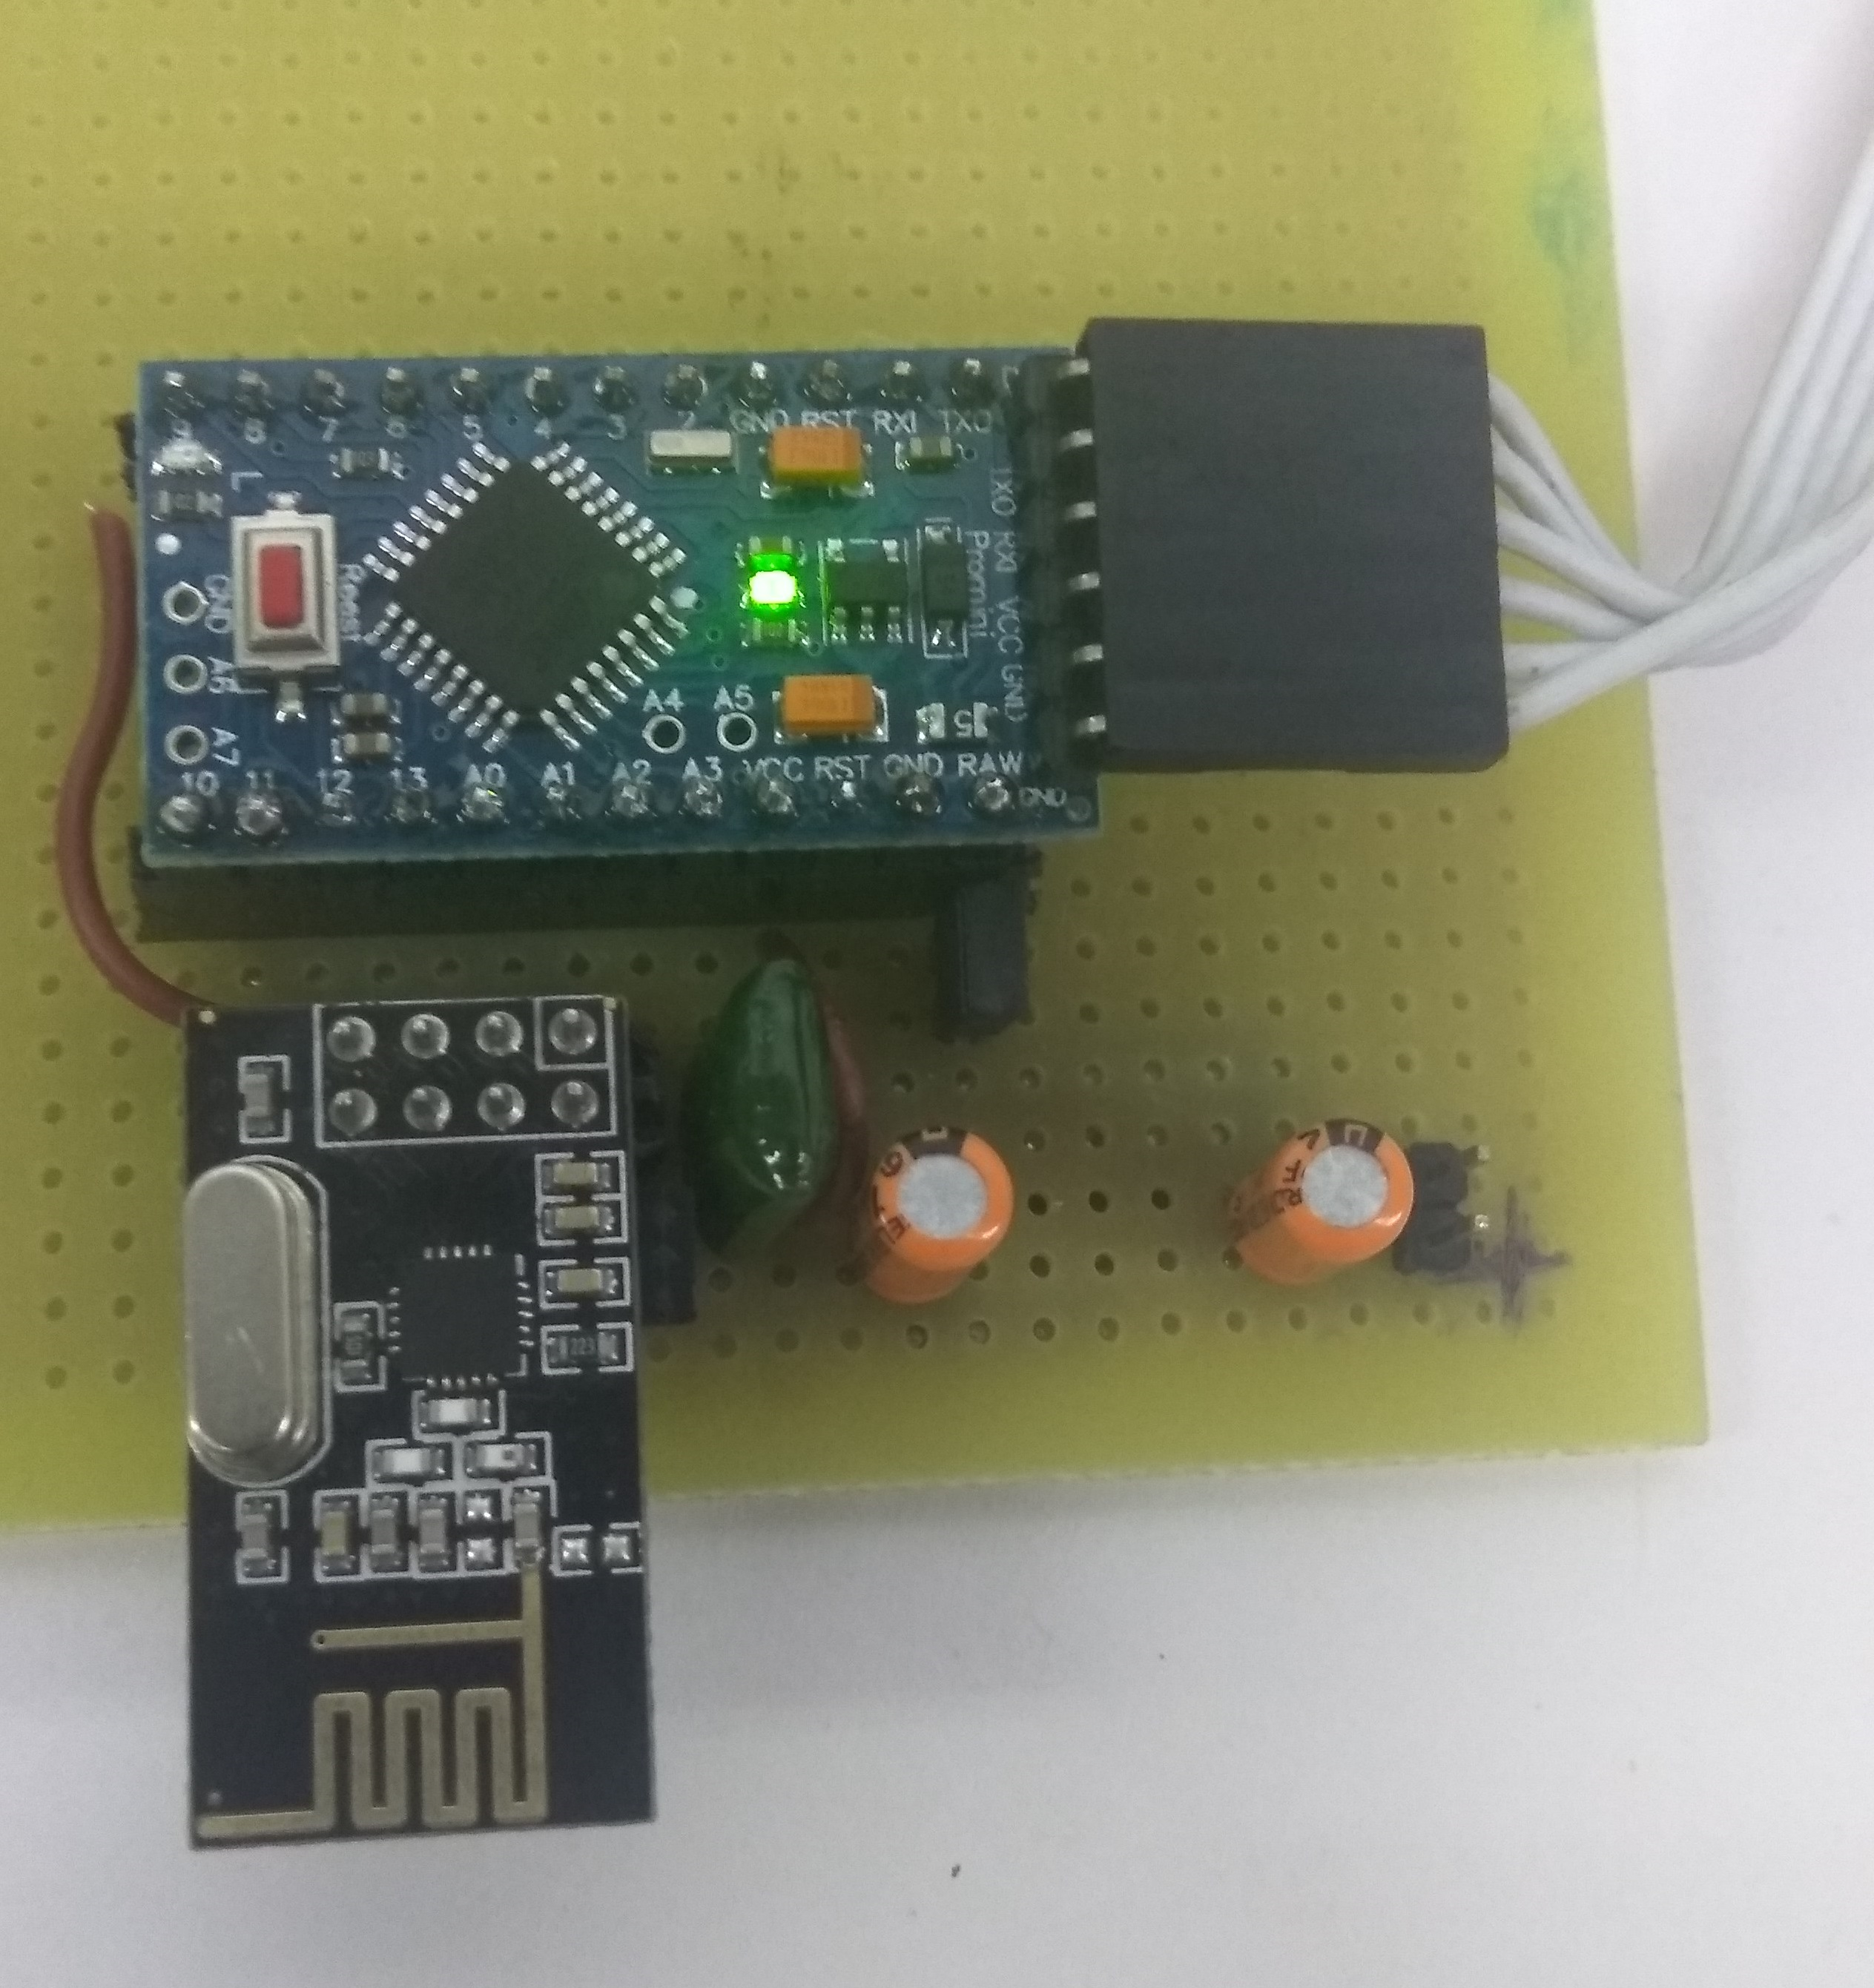
\includegraphics[width=0.9\textwidth]{hardware_prototype.PNG}\\
         \small{Figure 6\textbf{. Implementation of handmade prototype model}}\\
\end{center}
\clearpage
\begin{itemize}
\item Printed PCB hardware of Node
\end{itemize}

\begin{center}
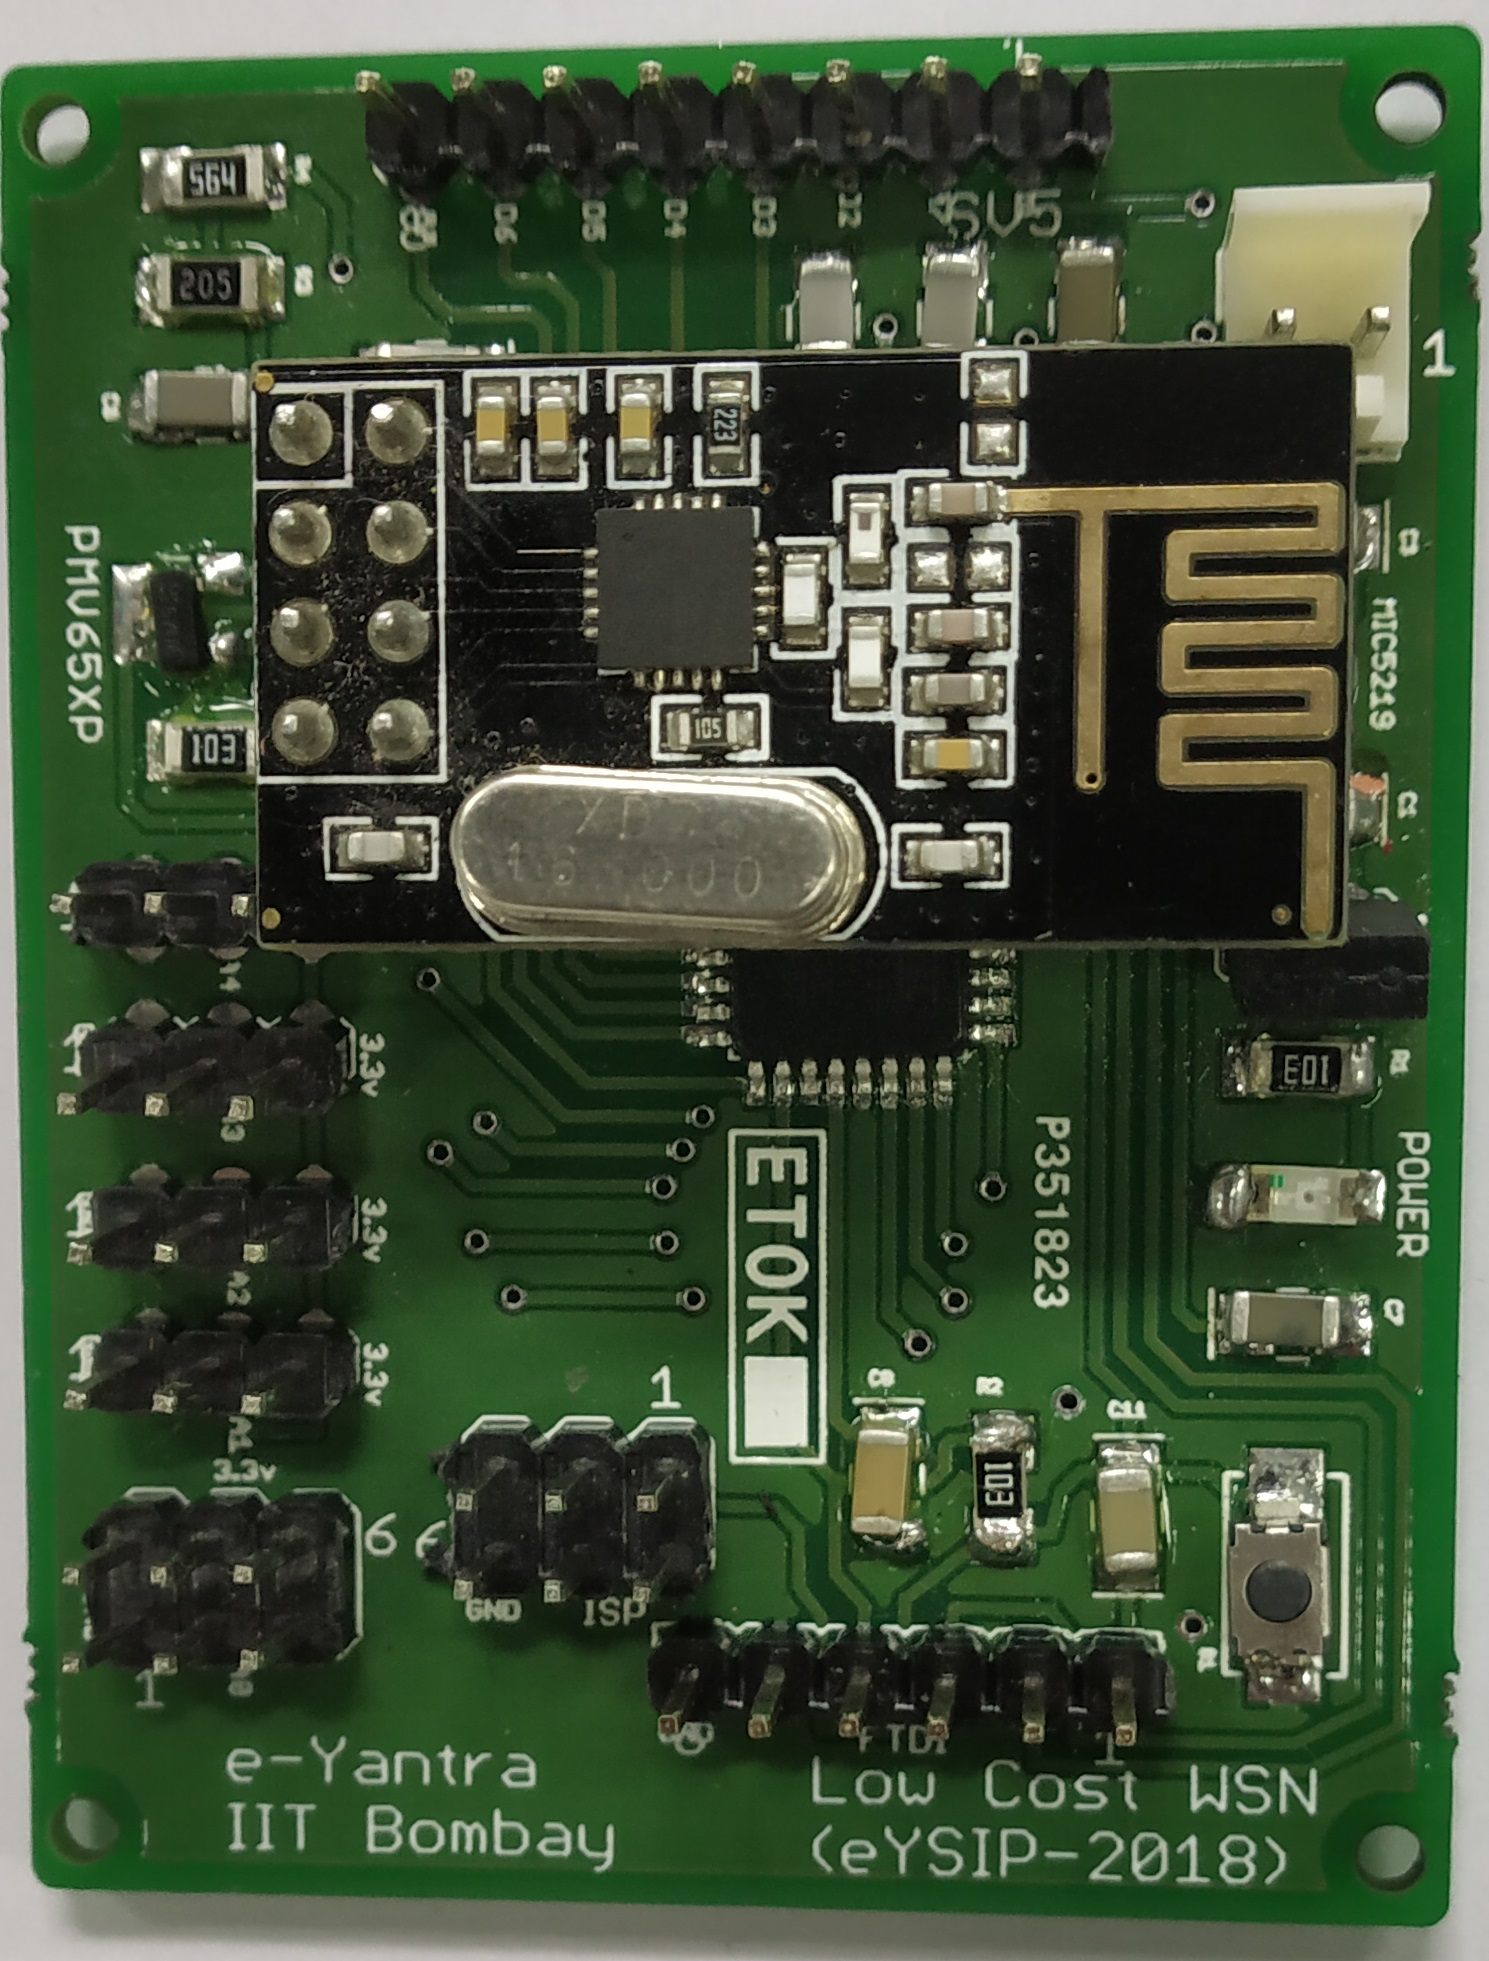
\includegraphics[width=0.5\textwidth]{node_Printed_board.PNG}\\
         \small{Figure 7\textbf{. Printed PCB of node}}\\
\end{center}

\begin{itemize}
\item Pin configuration and connection 
\end{itemize}
\begin{center}
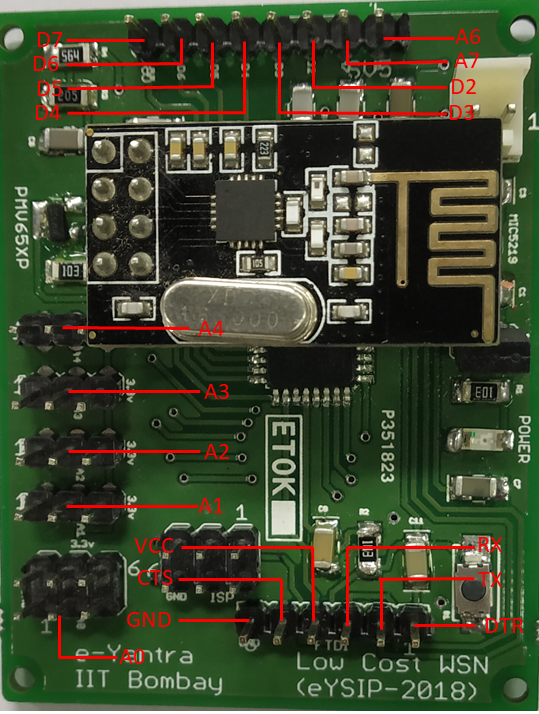
\includegraphics[width=0.45\textwidth]{pinout.PNG}\\
         \small{Figure 8\textbf{. Pin configuration of board}}\\
\end{center}


\begin{center}
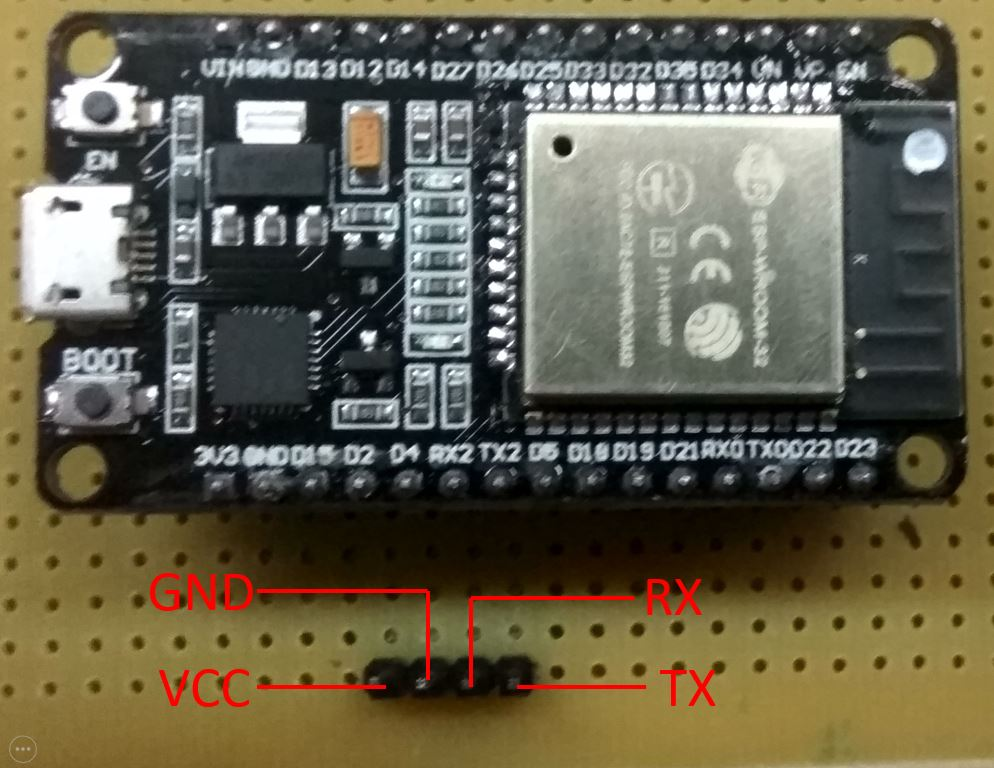
\includegraphics[width=0.5\textwidth]{pinout_1.PNG}\\
         \small{Figure 9\textbf{. Pin out connection of ESP32}}\\
\end{center}

\begin{itemize}
\item Here we implemented a star network in which there was three transmitters and one receiver were the receiver node was said to be a hub of the whole network which is connected to ESP32 gateway for uploading the received data to the thingspeak server.

\end{itemize}
\begin{center}
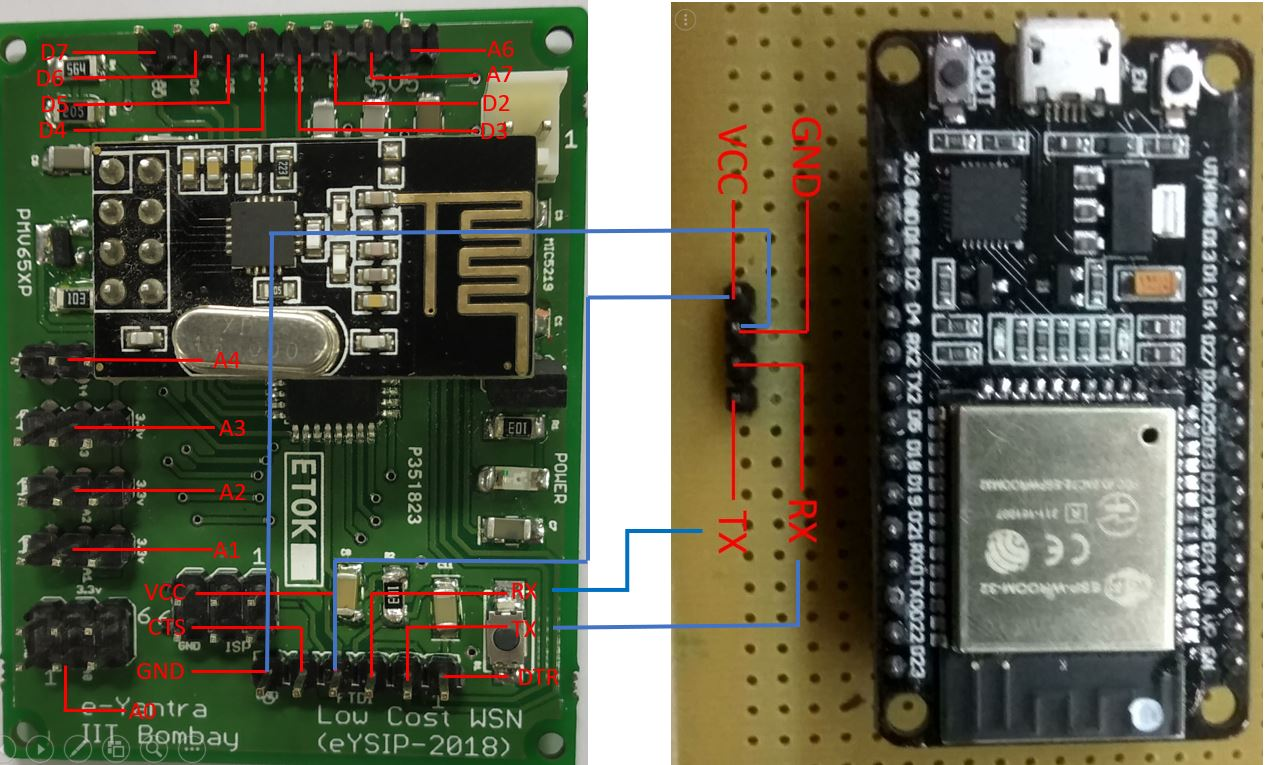
\includegraphics[width=0.5\textwidth]{gateway.PNG}\\
         \small{Figure 10\textbf{. Connection description of hub and ESP32}}\\
\end{center}




\section{Software and Code}
For the repository of code \href{https://github.com/eYSIP-2018/Low_Cost_Sensor_Node} {Github link}

Brief explanation of various parts of code 

\section{Use and Demo}
Final Setup Image

User Instruction for demonstration

\href{https://github.com/eYSIP-2018/Low_Cost_Sensor_Node}{Youtube Link} of demonstration video 

\section{Future Work}
\begin{itemize}
\item We have implemented two types of network star network and mesh network which consist of 3 transmitting nodes and one receiver node usually known as a Hub. This implementation can be extended more by implementing a hybrid network which is a combination of star network and mesh network.
\item  JSON packet can be used for uploading bulk data to the thingspeak cloud. So that it can replace the current method of uploading data to the cloud which is sending a post request to the server. 
\item The onboard LED must be connected on D13 pin for debugging of NRF data receiption \& transmission.
\end{itemize}

\section{Bug report and Challenges}

\begin{itemize}
        \item Prototype testing of nRF24L01
        \begin{itemize}
        \item In the starting days we were connecting nRF24L01 with Arduino pro mini via one to one connectors so we were facing loose connection and sometimes due to some fluctuations in the voltage the nRF24L01 was not giving appropriate reading. So we implemented an hardware on which we carried out our testings which mitigated our fluctuations and loose connection problem.
        \end{itemize}
        \item Range testing of nRF24L01 in outdoor environment
        \begin{itemize}
        \item After implementation we took our prototype model for testing it at the terrace of KReSiT building as there are lot of Wi-Fi connections available at the terrace so it was creating lot of disturbance in the communication as Wi-Fi so we used 76 channel number for  using radio frequency as nRF24L01 works on 2.4 GHz frequency greenery present over there was absorbing 2.4 GHz frequency up to some level.
        \end{itemize}
        \item Setting of fuse bits (Low, High, Extended) using AVRDude
        \begin{itemize}
        \item While setting fusebits we were facing some problem for setting it initial and also reading the fusebits. Finally we found that commands we were using was having some error  in it so we used  a appropriate command for it and it worked well.
        \item At starting we are using FTDI chip for modifying fuse bits through serial communication,but  Fuse bit and lock bits can not be changed through serial communication i.e. through FTDI chip. so after that we have used stk500v2 programmer which uses SPI to acess direct flash and usig proper commands for writing fuse bits in AVRDUDE problem is solved.
        \end{itemize}
        \item Importing RF24 library in Atmel Studio
         \begin{enumerate}
         \item RF24.h is made for any arduino device along with ESP \& R-PI.For this is using arduinocore i.e.arduino.h , SPI.h ,Each library of  approx thousands of lines.
         \item So first of all i am not getting where to start . Then I have started step by step.\begin{itemize}
         \item Listed down all the functions used by RF24.cpp from arduino.h same for SPI.h
         \item Written all this function in Embedded C and added GPIO.h file and GPIO.c file in same folder in SPI.h and RF24.h and removed Aduino.h
         \item There are lot of unnecessary macro which are not needed for Atmega328p in RF24.h , SPI.h  all of this modified properly.
         \end{itemize}
         \item For proper SPI speed and settings I have rewritten the \textbf{SPI.h} library at register level referring from Atmega328p datasheet.
         \item After doing this, Project Compiled successfully but nrf is not receving data.Because for reading the NRF pipe addresses and it needs some proper macros to be defined to read data from Program Flash memory with \textit{pgmspace.h} included.
         \end{enumerate}
   
        \item Differentiating data of multiple transmitter at one receiver
        \begin{enumerate}
        \item Differentiating data from multiple transmitter in star network
        \begin{itemize}
        \item We faced problem while receiving data from multiple transmitters to identify which data belongs to which transmitter so to solve this problem we used a pipenum function which will provide the pipe number from which it has received the data. By using pipe number we were able to differentiate multiple data's of different transmitters but this worked only in the star network.
        \end{itemize}
        \item Differentiating data from multiple transmitter in mesh network
        \begin{itemize}
        \item While implementation of mesh network we faced the same problem as in the star network of differentiating different data at the receiver end. So for this problem we used a string data who's first character will consist of the node ID or address of the transmitter data which is parsed at the receiver end for identification of the node ID which is send along with the transmitted string.
        \end{itemize}
        \end{enumerate}
		\item Importing C file in C++ ATMEL project.
        \begin{itemize}
        \item The gpio library written in .C and project main file is in .cpp format , so while using function form .C inrary in main the error is "Undefined refrence to function".
       \item This is because Name mangling of compilers , linker can not link files with diffrent symbols . Compiler creates two diffrent symbols for same function in diffrent because of function oerloading in C++.
       \item This bug is solved by including gpio.h header file inside extern "C" command which disables name mangling for functions unside that .h header file and treat it as a C file.
        
        \end{itemize}
        \item Timing issue with SPI library
        \begin{itemize}
        \item After sending data through MOSI pin and then making NRF24L01+ as RX or TX  CE pin written with low and high value respectively.
        \item After writing level value to pin it needs some time to stable and that much time MCU needs to be wait . so I have find that time for NRF24L01+ for its datasheet.
        \end{itemize}
        
        \item Transmit and Receive float value in string 
        \begin{itemize}
        \item While transmitting a float data from the transmitter it was not able transmit float data from it. So we converted float data into character and stored it into string  for sending it.
        \end{itemize}
        \item Synchronization in Star network with duty cycling on both sides
        \begin{itemize}
        \item We searched for diffrent protocols for synchronization like \textbf{RBS,TPSN,FTSP}.
        \item Tried by flooding method in which Recevier hub sends some count value to each node and for that much count value that particular node goes in sleep and after sending all count value recevier goes into sleep for the count value which is minimum and after that it will wake up to take data form first node.
        \item Tested with one transmitter and one receiver worked fine by putting both the TX \& RX in sleep.
        \item While implementing with more than one node it is not working with that much of accuracy because sometime it happens like node is transmitting but receiver in sleeep at that time \& vice versa.One as for flooding each Node be a used as transrecevier with its own address properly but because power down timing accuracy some cases arises like all the node are in transmitting and nomone is listening and vice versa also.
        \item So for this method we need a global clock that we don't have so we kept receiver continuously on and did duty cycling using power down API at each node.
        \end{itemize}
        \item Serial communication between arduino nano(hub) and ESP32
        \begin{itemize}
        \item While sending data from hub to ESP32 gateway we opt to transmit data serially from hub to gateway while doing that we faced lot of problems  for synchronization of both. So we solved it by sending an acknowledgement from gateway to hub as soon as the data is received at the gateway side from the hub and also it will send a character while it gets connected to the available Wi-Fi network. So that hub can send data to it and esp32 is ready to receive data from it.
        \end{itemize}
        \item It was a very tough challenge to upload bulk data to thingspeak server at once. 
        \begin{itemize}
        \item While uploading data to the thingspeak server the main challenge was to upload multiple channels in a single instant and to view it on the same screen. So we tried to upload multiple data to multiple channels of the thingspeak server but by doing so data cannot be viewed on a single screen so we uploaded different data's to different fields of the GUI. So that we can easily view all the uploaded data on a single screen.
        \item Also we tried to implement JSON packet for uploading bulk data to the server but it didn't worked perfectly.
        \end{itemize}
        \item After completing soldering of all smd components on the printed pcb it was ready to be implemented, while implementing it we found a hardware issue which was all about the LDO and its capacitor combination, we were using a non polarized capacitor, which was not that capable to fulfill the need of the whole pcb. So the problem was solved by replacing the non polarized capacitor with a polarized capacitor.
        \begin{center}
          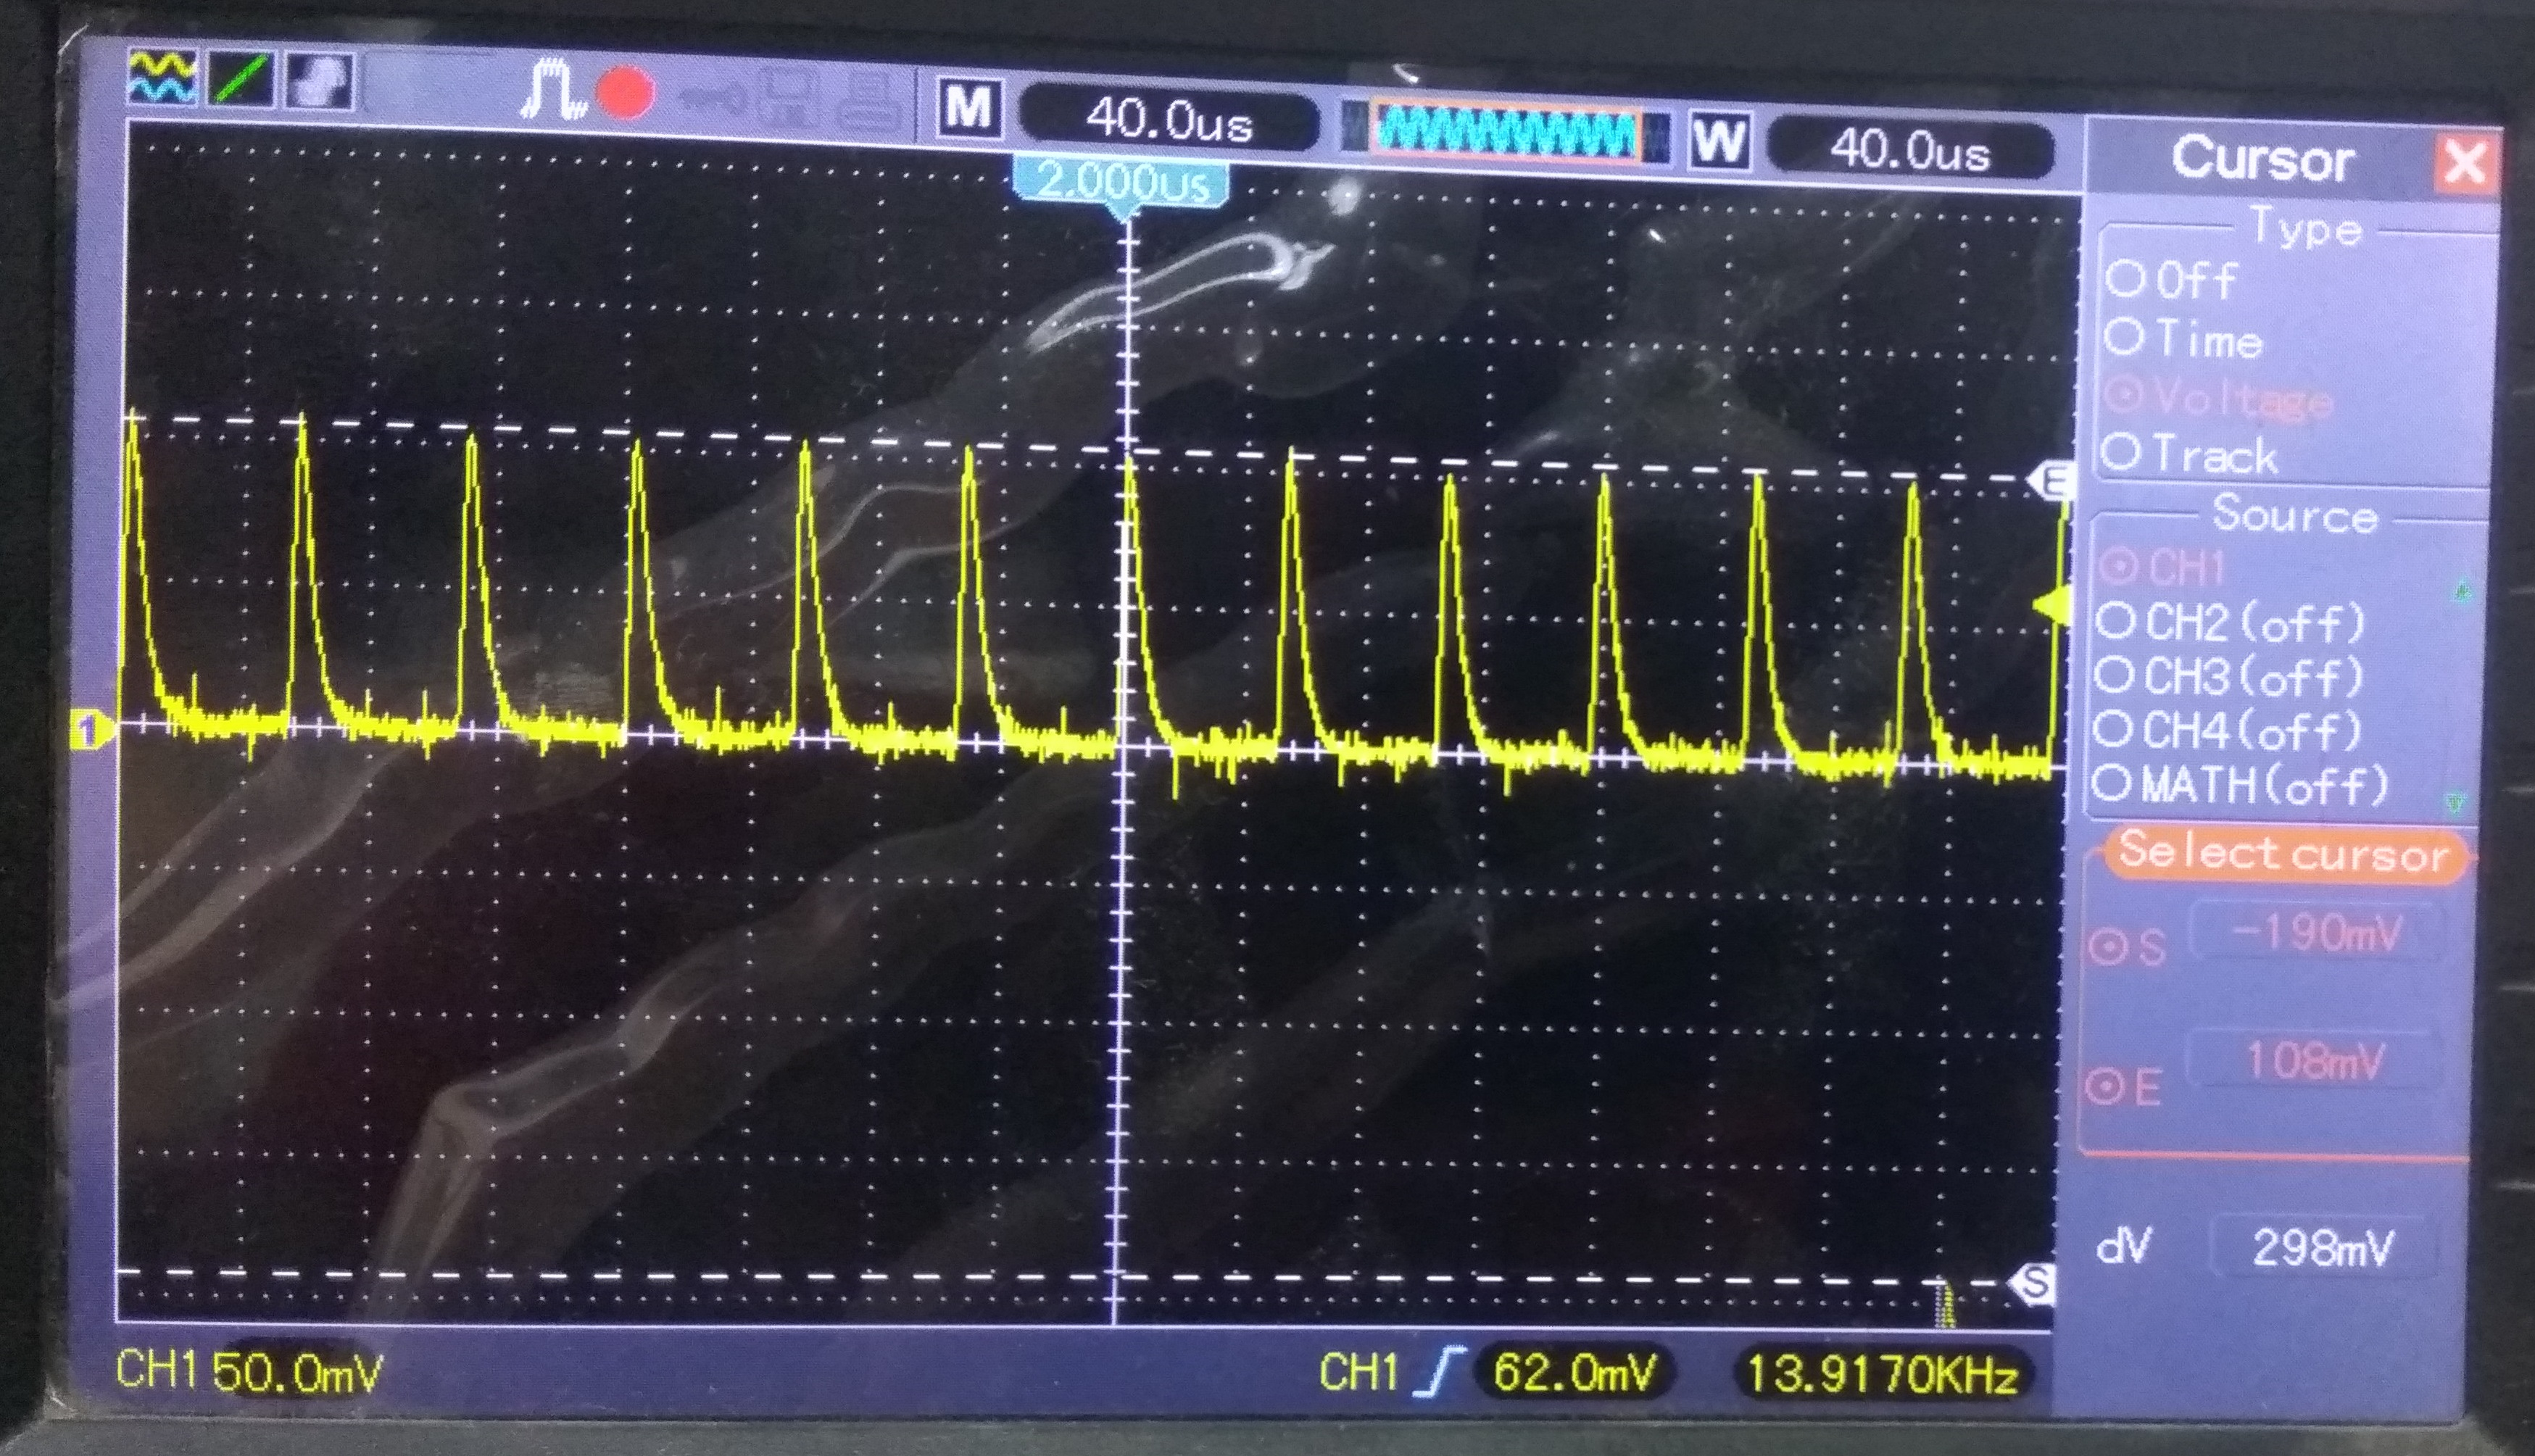
\includegraphics[width=0.7\textwidth]{deltavoltage.jpg}\\
          \small{Figure 11\textbf{. CRO reading of change in voltage w.r.t. time}}\\
          \end{center}
          \item The above figure shows that the change in voltage with respect to time of  CRO reading which we obtained.
 \item MOSFET Switching on Board
 	\begin{itemize}
 	\item The bug is the code/api for initializing of NRF24L01+ is outside the while 1 loop ,and after that MOSFET switching is done.
    That is at the time of initialization nrf is not powered and because of nrf is not receving/transmitting data properly.
    \item Switch on MOSFET outside while 1 loop and then call the API's of initialising of NRF24L01+.
 	\end{itemize}

	\end{itemize}

\begin{thebibliography}{li}
\bibitem{wavelan97}
Sachin Gajjar, Nilav Choksi, Mohanchur Sarkar and Kankar Dasgupta,
{\em Comparative analysis of
Wireless Sensor Network Motes},
2014.
\bibitem{wavelan97}
Ad Kamerman and Leo Monteban,
{\em Low cost wireless sensor networks for environment monitoring}, 2015.
\bibitem{wavelan97}
ZHU Jian-hong, WANG Jun and LIU Di,
{\em Design of A Wireless Sensor Network Node Based on nRF2401}.

\bibitem{wavelan97}
Sergey Y. Yurish, Javier Cañete and Francisco Puerta,
{\em Cost-effective Sensor Nodes for Wireless Sensor Networks}, 2012.

\bibitem{wavelan97}
S. S. Sonavane, V. Kumar and B. P. Patil,
{\em Designing Wireless Sensor Network with
Low Cost and Low Power}.

\bibitem{wavelan97}
Vidyasagar Potdar, Atif Sharif and Elizabeth Chang,
{\em Wireless Sensor Networks: A Survey}, 2009.

\bibitem{wavelan97}
Rajinder Kumar Math and Nagaraj V Dharwadkar,
{\em A Wireless Sensor Network Based Low Cost and
Energy Efficient Frame Work for Precision
Agriculture}, 2009.
 
\end{thebibliography}


\end{document}
-